%% ----------------------------------------------------------------
\chapter{Implementation - Payload}
%% ----------------------------------------------------------------


\section{Overview}
||||||| Might not want this in its own section ||||||||

The payload controller module is an important part of the system, responsible
for interfacing with the camera module and communicating with the ground 
station image viewer software via the autopilot. Since this single module 
encapsulates a significant amount of the complexity of the project it was 
deemed sensible to split it up into sub-modules, which could be worked on in
parallel by different members of the team. 

With this in mind the payload controller module was split into four main 
submodules:

\begin{itemize}
	\item Camera Module Communication
	\item Communication with Ground Station via Autopilot
	\item SD Card Image Buffering
	\item Progressive JPEG Manipulation
\end{itemize}

||||||| INCLUDE REFERENCES TO EACH ||||||||||

||||||| INCLUDE SUBMODULE DIAGRAM OF THE PAYLOAD MODULE |||||||

\subsection{Camera Module}
\label{sec:John_Implementation}

The first step in the implementation of the camera module was to verify the communication with the camera by talking to it via a pc. Once this step was complete the next step was to implement communications between the camera and a microprocessor, with the pc for debugging. With the microcontroller able to communicate with the camera this module was ready for integration with the payload.

\subsubsection{First camera}


\section{Communication with Ground Station via Autopilot (mh)}
\label{sec:payload controller}
Considering the overall aim of this project: to produce a system by which 
images can be downloaded over-the-air from a payload module to a ground 
station, some method of communicating between the
payload module and ground station are an essential component in the system.

The specification requires the payload
module to communicate with the ground station using the autopilots payload
module interface (discussed in section \ref{sec:autopilot_payload_interface}).

%To better explain the protocol used we will split the explanation into two 
%sections: a \emph{Autopilot Payload Interface} section describing the
%pre-existing autopilot payload interface on which we are building the 
%protocol and a \emph{UAV Camera Communication Protocol} section describing the 
%protocol we have implemented as a part of this project.

\subsection{Existing Code}
\label{sec:payload_existing_code}
Our customer had provided us with some payload module communication AVR code
- written for a ATMega168 - for communicating with the autopilot. This code
was the basis on which the payload controllers communication link was built.

The code provided a number of useful utilities:
\begin{itemize}
\item Basic connection to the autopilot, including responding to transmit tokens.

\item Ability to set shared memory on the autopilot.

\item Ability to receive messages sent from the Ground Station to the 
autopilot.

\item Example code for setting shared memory on the autopilot.
\end{itemize}

This base code was modified slightly after a bug was found in its handling of 
the transmit enable signal. The RS485 communication protocol used for the 
autopilot-payload link (as described in section |||||||| SEC ||||||||) 
requires a `transmit enable' signal to be asserted when the payload is 
transmitting. This signal should be asserted just before data is to be sent 
and cleared just after. However, the original payload base code cleared this 
signal in an interrupt service routine (ISR) which fired after the transmit 
buffer of the UART was ready to accept new data. Since this transmit buffer 
would be ready to accept new data before the data was actually sent over the
physical connection this lead to the transmit enable signal being cleared
before all data had been sent, causing strange behaviour on the RS485 link.
This bug did not seem to cause any problems, and the odd behaviour was only
noticed when testing the system with an oscilloscope. ||||| INC TRACES ||||||
It was considered sensible to fix the bug in case it did cause problems later.

The fix for this problem was reasonably simple: a new ISR was set up which 
fired only when the current transmission had actually completed, and the 
command to clear the transmit enable signal was moved into this ISR.
||||| INC AFTER TRACE ||||||

\subsection{Establishing Contact with the Autopilot (mh)}

The first step in implementing the communications link was to establish contact with
the autopilot using the existing module code, the relevant milestone being
\ref{sec:ms_pl_tx_token_resp}. 

A problem was encountered during this step where the payload would not 
respond to a transmit token in any way. Debugging this problem with a 
oscilloscope showed that the autopilot was not sending transmit tokens.

After spending some time ruling out problems with our own design that could be
causing this, including looking at the RS485 chip in case it was conflicting with the
autopilots serial bus or malfunctioning, we contacted our customer and queried 
whether it could be a problem with the autopilot itself, presenting our evidence of
debugging.

Our customer responded by acknowledging that it was a problem with the autopilot
and providing us with an updated firmware for the autopilot
which would send the transmit tokens correctly.

After this bug was fixed the payload responded as expected, 
section \ref{sec:test_pl_est_contact} describes the successful testing of this part of
the implementation.

\subsection{Setting Shared Memory on the Autopilot (mh)}
Once basic contact had been established the next task was to set shared memory on
the autopilot - as per milestone \ref{sec:ms_pl_shared_mem_set}. The existing code
provided allowed this to be completed quickly using the built in functions. Section 
\ref{sec:test_pl_set_shared_mem} details the tests carried out to validate this
was working.

\subsection{Recieving Messages from the Ground Station (mh)}
It was important to ensure that the payload recieved messages correctly from the ground
station before continuting with the implementation of this section, the customers provided code
allowed this to be completed quickly also. Section \ref{sec:test_pl_receive_message} describes 
the steps taken to test this.

\subsection{UAV Camera Communication Protocol (mh)}
As discussed in section |||||||| REF |||||||| it was decided that 
our communications protocol would use shared memory and \emph{send\_bytes} 
commands, allowing two way communications between the payload controller and 
ground station software to be established. With the ability to receive and send data
with these messages tested as described above, implementation could now begin on
implementing a communications protocol used to talk between the our ground station 
image viewer software and the payload.

The method through which this shared memory is accessed via the ground station
image viewer is discussed in chapter \ref{chap:implementation_ground_station}.

%The Payload Module Interface discussed above (section \ref{sec:autopilot_payload_interface})
%allows us to send strings of bytes in both directions. However, in order to 
%communicate with the ground station image viewing software some form of 
%additional communications protocol is required so that both ends of the link 
%are communicating in a mutually understandable manner.

This two way communications is the interface between the payload and the 
ground station software, so some standard protocol was required. It was decided
that a message based system would be used, with the messages from the ground
station to the payload module being sent using \emph{send\_bytes} and the 
messages sent from the payload to the ground station being put into shared
memory. Each message is composed of two elements, one byte for the message ID 
- unique to each type of message - and a variable number of data bytes 
(depending on the message type.) The different message types are detailed 
below:

\subsubsection*{Messages sent from Ground Station To Payload}

\begin{itemize}
\item \textbf{Take Picture}
\begin{itemize}
\item \emph{Data:} None
\item Prompts payload module to capture an image and save it to the SD card.
\end{itemize}

\item \textbf{Image Download Request} 
\begin{itemize}

\item \emph{Data:} Image ID
\item Requests the payload send the image with ID \emph{Image ID} to the 
ground station. This message allows any image stored by the payload module 
to be downloaded over the connection, increasing flexibility. 
\end{itemize}

\item \textbf{Configure Camera}
\begin{itemize}
\item \emph{Data:} Colour Type, Raw Image Resolution, JPEG Image
Resolution
\item Sets the image resolution and colour mode of the camera. Only the 
JPEG mode has been tested so far.
\end{itemize}

\item \textbf{Cancel Download}
\begin{itemize}
\item \emph{Data:} None
Resolution
\item Cancels the current download taking place.
\end{itemize}

\end{itemize}

\subsubsection*{Messages Sent from Payload to Ground Station}

\begin{itemize}

\item \textbf{Picture Taken}

\begin{itemize}
\item \emph{Data:} Image ID

\item Informs the ground station software that an image has been taken and 
saved to the SD card. \emph{Image ID} is the ID of the image that has been 
saved to the SD card.
\end{itemize} 

\item \textbf{Image Download Info}

\begin{itemize}

\item \emph{Data:} Number of Image Packets

\item Sent by the payload after a successful \emph{Image Download Request}
message from the ground station. Informs the ground station how many 
\emph{Image Data} packets to expect.
\end{itemize}

\item \textbf{Image Data} 
\begin{itemize}
\item \emph{Data:} Packet Number, Image Data
\item This message contains an amount of actual image data. Sent after a
\emph{Image Download Info} message which is in turn in response to an 
\emph{Image Download Request} message. The whole image is sent over
\emph{Number of Image Packets} packets (as defined by the \emph{Image Download
Info} message.) \emph{Packet Number} informs the ground station which of these
packets the message is carrying. \emph{Image Data} contains the actual image 
data for this packet and is variable size, with a maximum size of 50 bytes. 
\end{itemize}

\end{itemize}

Implementing this communications protocol was a significant challenge and was a major
component of the payload module implementation. 

Our implementation for the payload follows an event loop style, where an initial series of 
steps are preformed initializing the camera and SD card, after which the code then enters a continuously
running loop which checks to see if any messages have been received from the ground station.

When a message is received from the ground station (as sent by \verb+send_bytes+ command) a switch-case
conditional structure then decodes which message had been sent and
initiates the appropriate function on the payload (for example calling the camera code to take a picture when sent
a \emph{Take Picture} command).

%One problem encountered during the implementation was that when attempting to set shared
%memory using the payload module, the send buffer implemented in the customer's existing code
%could fill up


The basic sequence for sending data from the payload controller to the autopilot is to use the utilities provided 
by the customers existing code to place messages into the autopilots shared memory to be accessed by the
ground station, as described earlier. Only one set of shared memory is used, and is overwritten every time 
a new message is to be sent from the payload controller to the ground station.
Other features such as configuration of camera resolution are implemented using this basic mechanism, figure \ref{sequence diagram} describes many the sequence diagram of the data transmission.


\begin{figure}[H]
\begin{center}
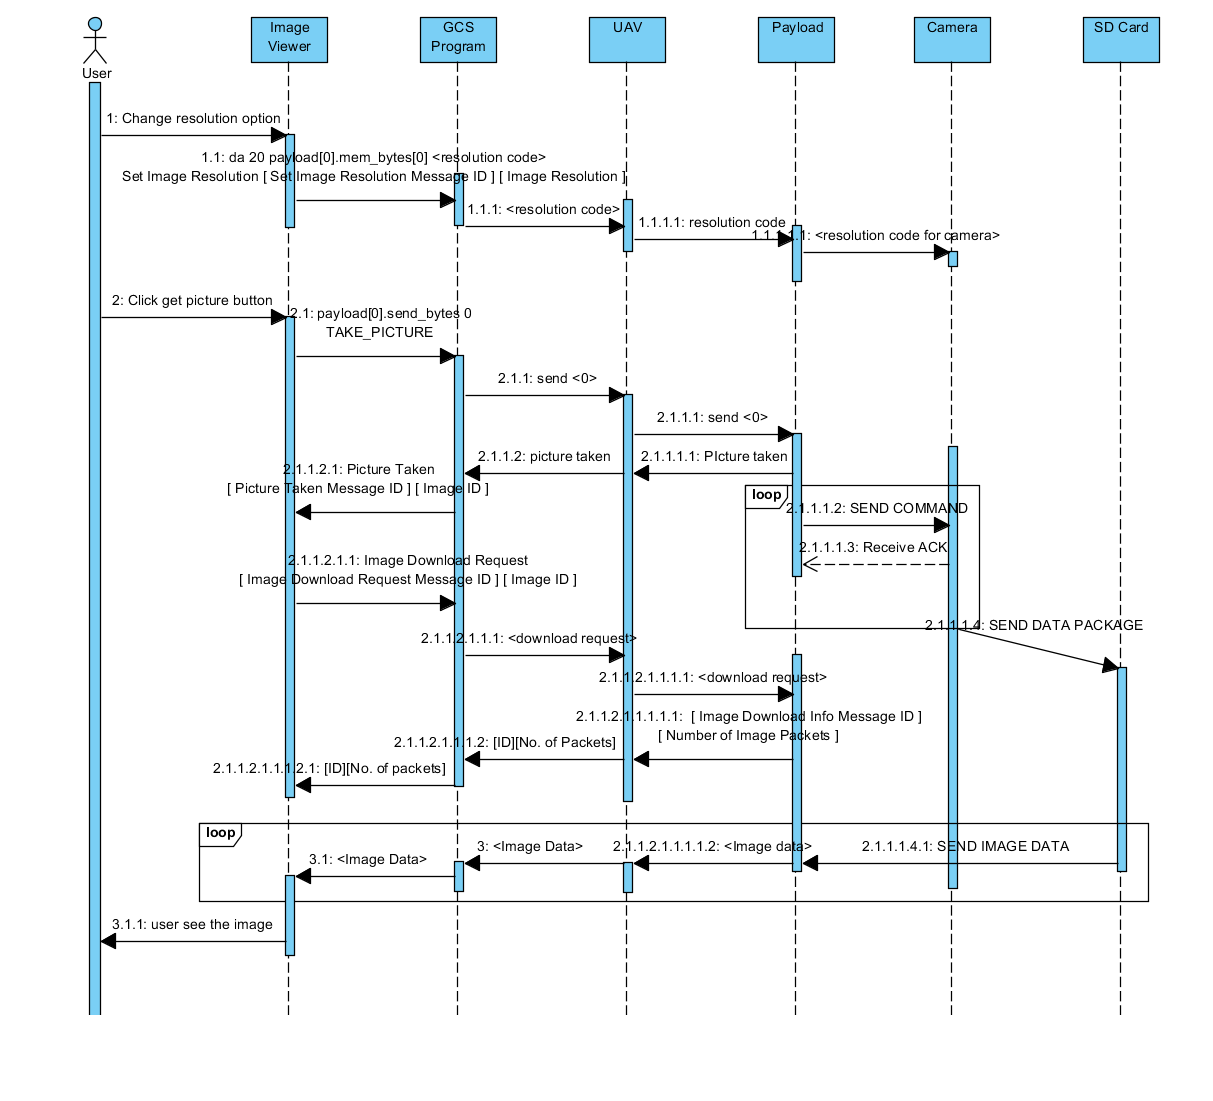
\includegraphics[width=1.00\textwidth]{figures/sequence_diagram.png} 
\end{center}
\caption{Sequence Diagram of the Data flow\label{sequence diagram}}
\end{figure}

Image data is also sent in the same basic manner, however the image is broken up into `packets' of data
which can be placed into the shared memory of the autopilot one at a time, as described by the \emph{Image Data}
message described above. One packet is sent for every transmit token sent by the autopilot, ensuring that the
payload module does not saturate the autopilot link with data. While packets are being sent, the main event loop
still checks for messages being sent from the ground station, allowing functionality such as the cancel download message 
to be implemented. In this way the payload module can transmit a whole image over the autopilot connection.

The testing of the image sending system is described in section \ref{sec:test_pl_image_send}, verifying the milestones 
as described.

Verification of milestone \ref{sec:ms_pl_img_gs_cam_res} (changing image resolution) can be seen in test \ref{sec:test_change_resolution}. Unfortunately changing colour type (milestone \ref{sec:ms_pl_img_gs_cam_colour_type})  was not fully implemented due to time constraints.

\subsection{Problems Encountered (mh)}
A number of problems were encountered and overcome during the implementation of the payload-ground station
communication code, a few of the most important are reproduced here.

\subsubsection*{Autopilot Bug (ab)}

The Autopilot sends "Transmit" tokens to the payload module every 20ms, 
to which a payload module sent an "ACK" token, even when it does not 
transmit any data. We encountered a problem whereby if our we tried to 
send any data to the payload during an "ACK", the autopilot would stop 
sending any "Transmit" tokens at all, effectively cutting off all 
communication to the payload module.

\begin{figure}[H]
  \centering
  \begin{tabular}{c c}
  \subfigure{\label{fig:testing_sc2_working1}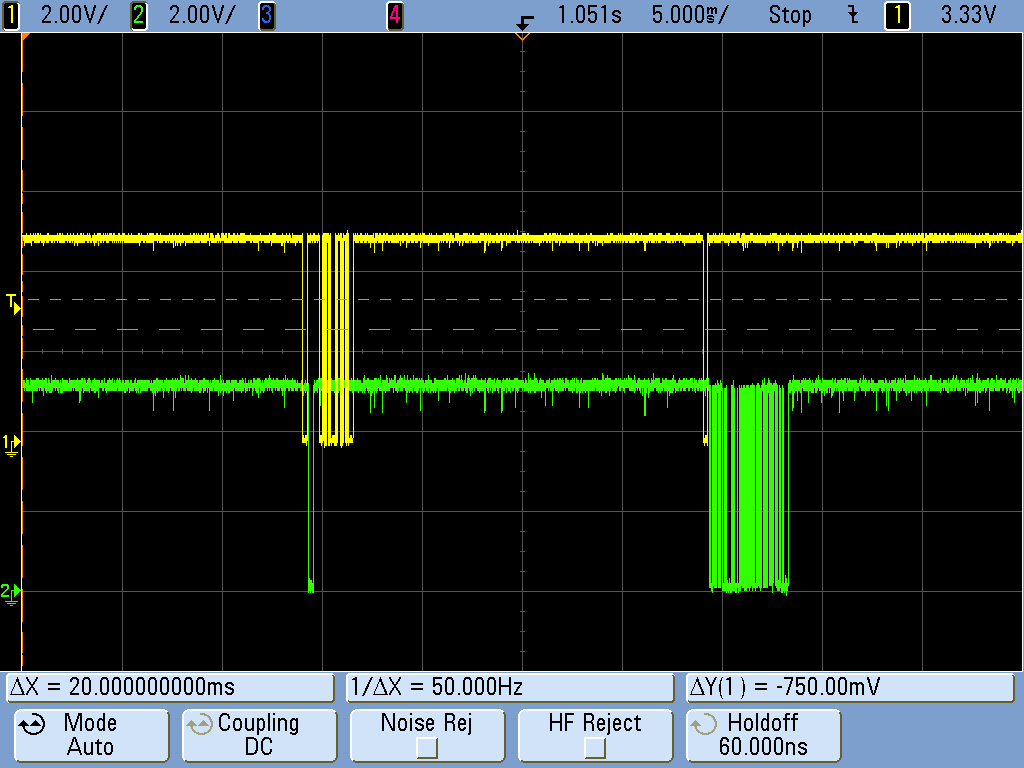
\includegraphics[width=0.5\textwidth]{scope/scope_1.png}}&                
  \subfigure{\label{fig:testing_sc2_working2}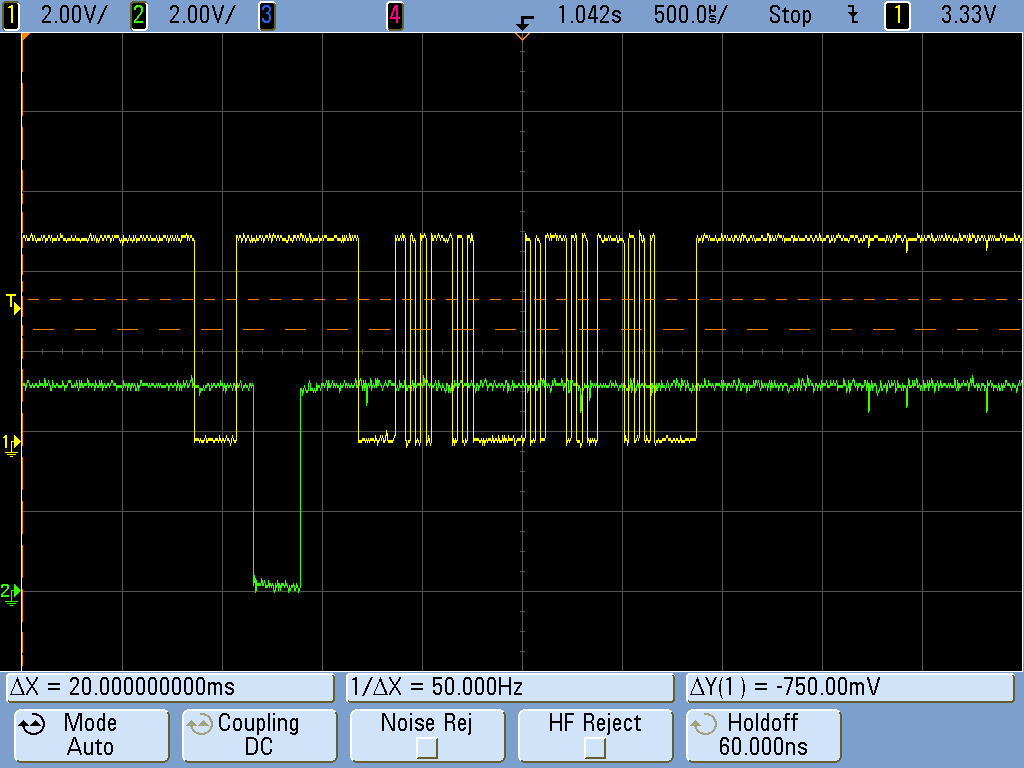
\includegraphics[width=0.5\textwidth]{scope/scope_2.png}} \\
  \subfigure{\label{fig:testing_sc2_working3}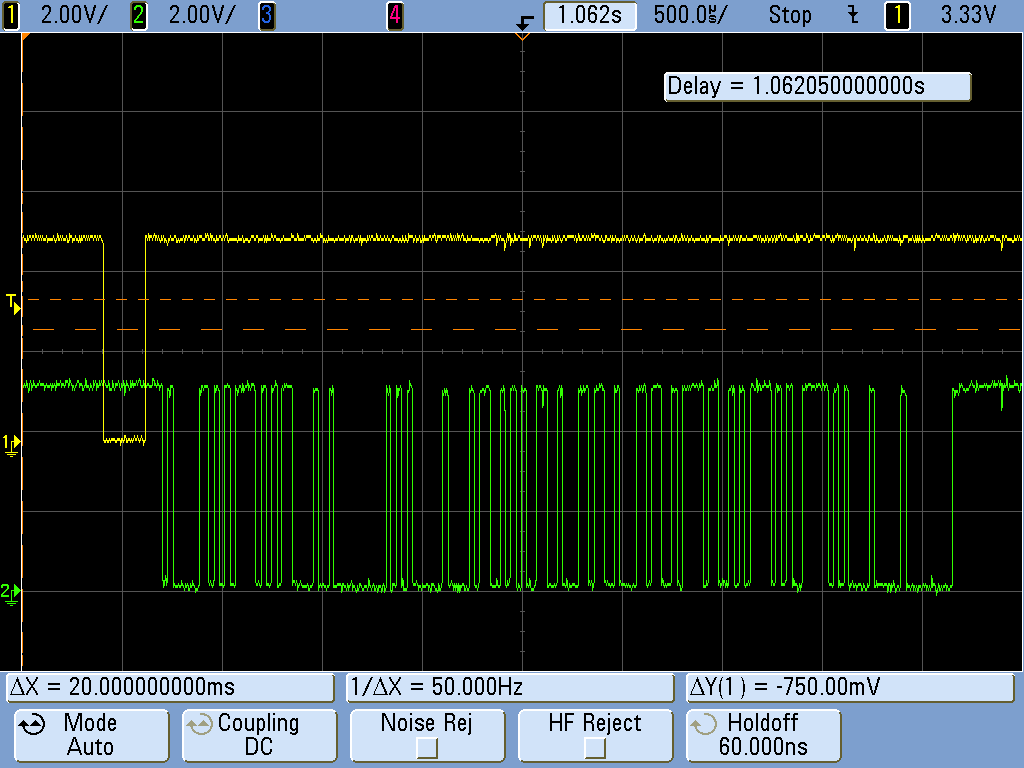
\includegraphics[width=0.5\textwidth]{scope/scope_3.png}}&                
  \subfigure{\label{fig:testing_sc2_working4}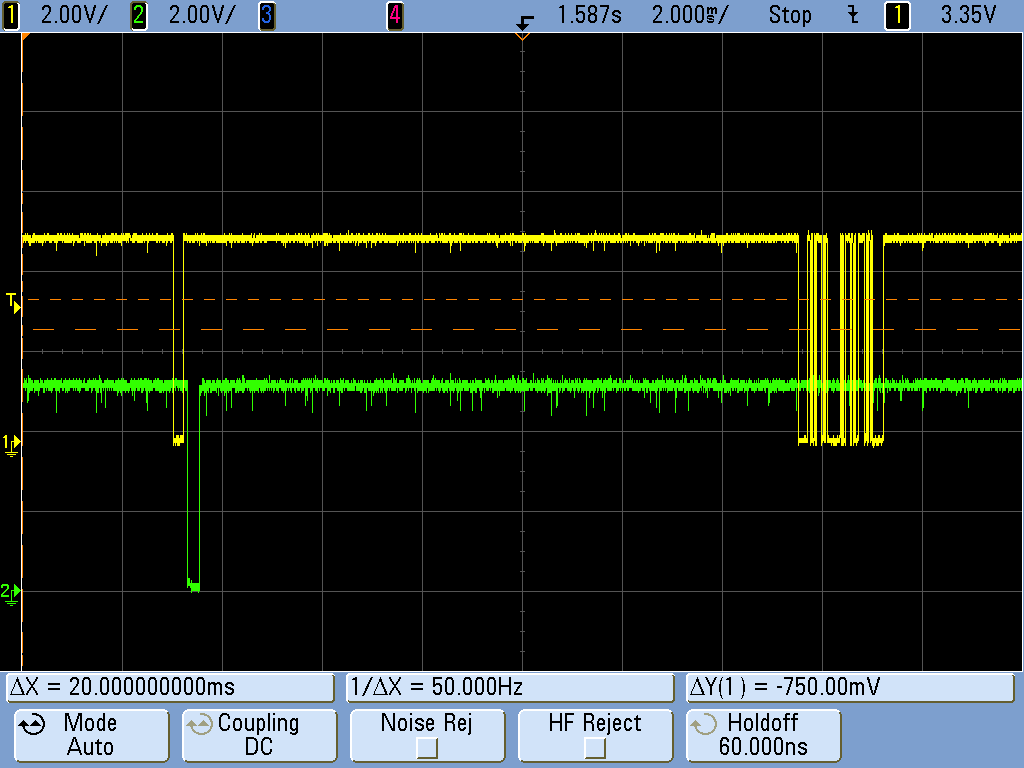
\includegraphics[width=0.5\textwidth]{scope/scope_11.png}}
  \end{tabular}
  \captionof{figure}{Oscilloscope traces for the situation where the autopilot does not break: In yellow is the Autopilot TX, in green the Payload TX. In this situation, after an ACK token is received by the autopilot, a SEND\_BYTES instruction is sent. On the next transmit token, a series of bytes is sent to the autopilot, and the autopilot continues to send Transmit tokens.}
  \label{fig:testing_sc2_working}
\end{figure}

\begin{figure}[H]
  \centering
  \begin{tabular}{c c}
  \subfigure{\label{fig:testing_sc2_broken1}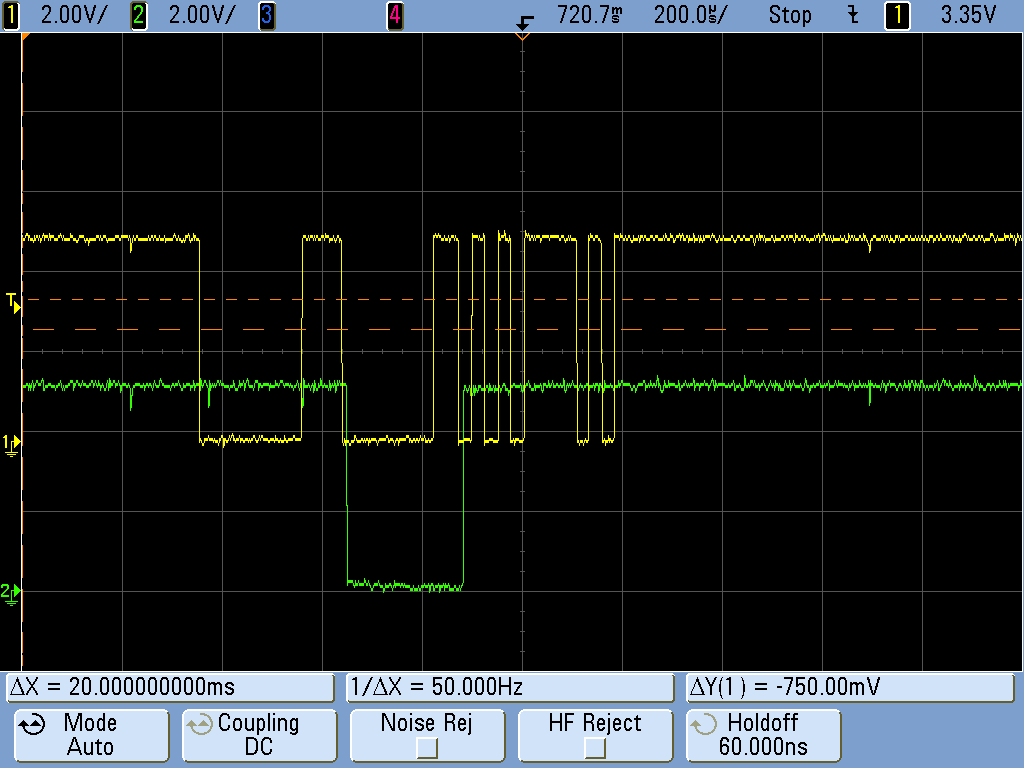
\includegraphics[width=0.5\textwidth]{scope/scope_6.png}}&                
  \subfigure{\label{fig:testing_sc2_broken2}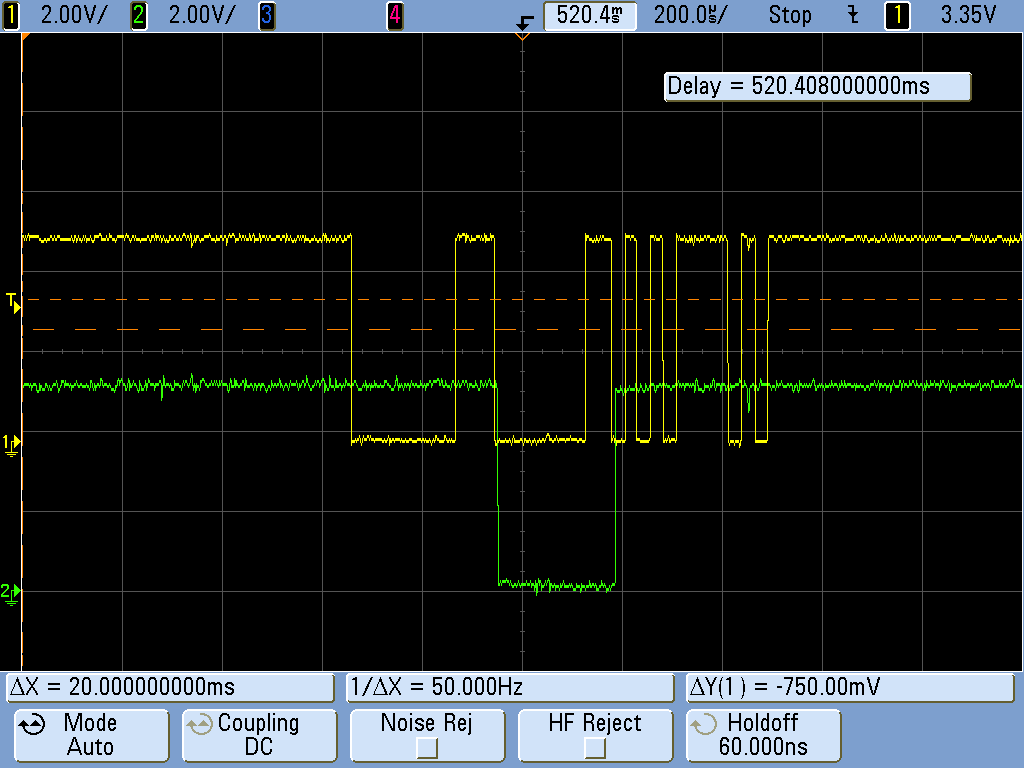
\includegraphics[width=0.5\textwidth]{scope/scope_14.png}} \\
  \subfigure{\label{fig:testing_sc2_broken3}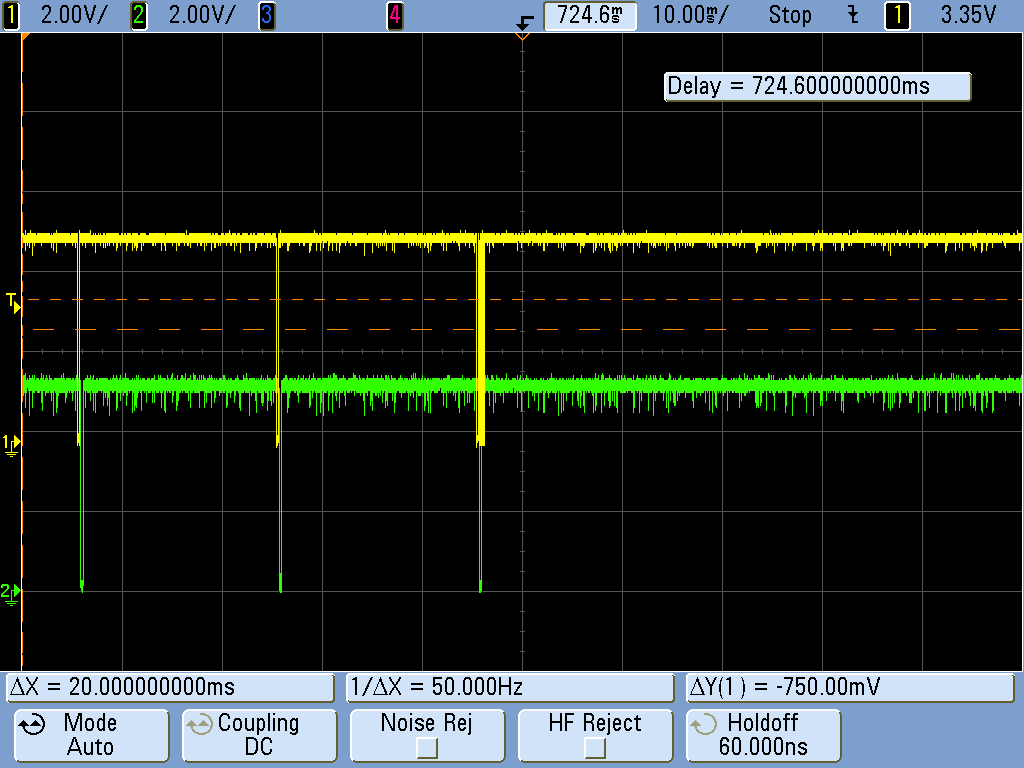
\includegraphics[width=0.5\textwidth]{scope/scope_7.png}}
  \end{tabular}
  \captionof{figure}{Oscilloscope traces for the situation where the autopilot breaks: In yellow is the Autopilot TX, in green the Payload TX. In this situation, whilst an ACK token is received by the autopilot, a SEND\_BYTES instruction is sent. No more transmit tokens are sent, therefore communication with the payload stops.}
  \label{fig:testing_sc2_broken}
\end{figure}

Not sure whether this was a bug with the Autopilot, we got in contact with 
our customer, sending all scope traces to him and a description of how 
to reproduce the error. Not being able to reproduce it with his dummy 
payload (strange, as our dummy payloads only differed in that his used a
surface-mount version of an ATmega168 and a MAX3070 transceiver instead 
of MAX489), he then came to ECS and debugged the Autopilot with us.

After a significant amount of time debugging the Autopilot and our 
payload, it was discovered this was indeed a problem with the Autopilot, 
which our customer was able to fix and subsequently update the firmware 
of our Autopilot.

\subsubsection*{Volatile Variables and ISRs (mh)}

Another problem encountered regarded a flag variable being checked in a function called in the main event loop. The flag
was the continuation condition of a while loop, and although it was being set in another section of code this new set 
value was not being propagated to the while loop code, meaning that the while loop would continue forever. This problem
was discovered (helped greatly by the debug interface described in section \ref{sec:payload_debug_interface}) . After some
consideration, research and experimentation it was discovered that the problem lay with the C compilers optimization. The 
flag was being set in a interrupt service routine (ISR), which the compiler assumed could not be called during the while loop
call, therefore it was optimized out, causing the loop to continue forever. The solution to this was to set this flag variable 
as \emph{volatile}, preventing it from being optimized out in this manner. The same was applied to all global variables modified in ISRs.


%|||||||| REMINDER: PROBLEMS CHALLENGES
%|||||||| REMINDER: HOW DID WE SOLVE PROBLEMS, DEBUGGING, TESTING, ETC
%|||||||| REMINDER: JOHN COULD TALK ABOUT HOW BROKEN CAMERAS SLOWED DOWN DEVELOPMENT BUT GOOD PLANNING AND CONTINGENCY MINIMISED RISK OR IN MANAGEMENT SECTION
%|||||||| REMINDER: FUTURE WORK
%|||||||| REMINDER: ADD NEWPAGES BETWEEN SECTIONS




\section{Progressive JPEG Manipulation}
\label{sec:implementation_progressive_jpeg}
The project planned to incorporate a custom JPEG manipulator which would
take a JPEG image received from the camera and progressively
send the image data to the ground station. 
The planned software would consist of two parts.

The first part of the software would obtain all the information
needed for reconstructing the JPEG image on the ground station.
This would be done using a JPEG image data extractor, and would 
also act to optimize the amount of information sent to the ground station.

The second part of the custom JPEG manipulation
would display the image progessively. 
This would receive the Huffman table information obtained 
from the extractor and use it to reconstruct the image progressively. 
It would then allow the user
at the ground station to evaluate the image as soon as possible,
i.e. before all the image data has been sent. This would also 
save time when combined with the ability to interrupt the 
downloading process of an image from the UAV to the
ground station in case the image appears to be unwanted. 

For information on the reasoning behind implementing 
custom JPEG manipulation, please see 
the JPEG manipulation section in the 
Approaches considered section. \ref{sec:jpegmanipulation}

During the course of the project, only the first part
of the progressive JPEG manipulation algorithm was 
successfully implemented. A form of image displaying 
software has also been constructed which uses the 
Huffman table information obtained from the extractor, 
but a progressively higher resolution display of 
the image was not able to be fully implemented.

\subsection{Progressive Scan of JPEG (commandCheck)}

After receiving the size of the JPEG file (in bytes), 
the JPEG Information Extractor starts reading the bytes of the JPEG stored in the SD card. 
Because the information will not all be available instantly, 
the extractor uses a class to read the next byte in the input stream, one at a time. This class \textbf{read\_byte()} is 
how the JPEG extractor gains access to the JPEG input stream. 

As the extractor reads in the bytes from the input stream, it checks to see if the byte indicates the start of a header (0xff). 
If this is the case, the next byte identifying the header is read and the \textbf{JPEGMethod} class is 
called which uses a switch command to determine the actions to take. 
If not, the data is discarded and the extractor continues to read the next byte is read from the input stream. 

\subsection{Image Data Extraction (JPEGMethod)}

The JPEG Information Extraction class does not need all the possible information that can be extracted from a JPEG image. 
The few image headers containing important information store the important information from the input stream into 
variables which will be sent to the custom encoding algorithm. 

If the header is not recognized by this class, 
it is assumed to not have any important information and is ignored; 
the code continues to scan through the input stream for the next header byte. 
The following headers have  information to be stored (all information is considered to be stored in one byte unless stated otherwise):

\paragraph*{SOF0: Start Of Frame (0xc0)}
\begin{description}
	\item[Data precision] indicates how many bits compose one sample (generally 8 to indicate a byte).
	\item[Image height] indicates the height of the image in pixels (2 bytes long).
	\item[Image width] indicates the width of the image in pixels (2 bytes long).
	\item[Number of components] indicates how many components define one pixel. 
		This will always be three for our cases to indicate the use of the YCbCr colour model. 
		The component information is read in in the order Y, Cb, Cr.
	\item[Component ID] indicates the ID number used by the JPEG file for this component.\footnote{One for each component}
	\item[Sampling factor] both horizontal and vertical are stored within a single byte. 
		The least significant 4 bits indicate teh vertical sampling factor, 
		while the most significant 4 bits indicate the horizontal sampling factor.\footnotemark[1] 
	\item[Quantization Table Number] associates the component to a quantization table.\footnotemark[1] 
\end{description}

\paragraph*{APP0: JFIF application segment (0xe0)}
\begin{description}
	\item[File Identifier Mark] indicates that this is a JFIF standard image.
	\item[Major Revision Number] must be checked to be 1.
	\item[Minor Revision Number] 
	\item[Units for x/y Density] 
	\item[X Density]2 bytes
	\item[Y Density]2 bytes
	\item[Thumbnail Width] Not used.
	\item[Thumbnail Height] Not used.
	\item[Remaining bytes] contains information regarding the image's thumbnail. This is not used in our extractor.
\end{description}

\paragraph*{DHT: Define Huffman Table(s) (0xc4)}
\begin{description}
	\item[HT Information] contains the following information concerning the indicated Huffman Table in one byte:
		\begin{description}
			\item[Bits 0\ldots3] ID number of the HT (cannot exceed 3)
			\item[Bit 4] Indicates whether the HT is DC (0) or AC (1)
			\item[Bits 5\ldots7] Unused.
		\end{description}
	\item[Number of Symbols] is a string of 16 bytes, each byte containing the number of symbols with 
		codes of length 1\ldots16. For example, if the third byte of the string is 7, 
		there are 7 signals of code length 3 in this Huffman Table.
	\item[Symbols] is a string of \emph{n} bytes, where \emph{n} is 
		the sum of all the values in the previous 16-byte string. 
		The extractor stores the Huffman tables in a linked list of struct objects representing the Huffman Tables.
\end{description}

\paragraph*{DQT: Define Quantization Table(s) (0xdb)}
\begin{description}
	\item[QT Information] contains the following information concerning the indicated Quantization Table in one byte:
		\begin{itemize}
			\item[Bits 0\ldots3] ID number of the QT (cannot exceed 3).
			\item[Bits 4\ldots7] Precision of the QT. Either 8-bit (0) or 16-bit (all other values).
		\end{itemize}
	\item[QT values] is a string of \emph{n} bytes, where \emph{n} is $64*$precision$+1$.
\end{description}

\paragraph*{SOS: Start Of Scan (0xda)}
\begin{description}
	\item[Number of components in scan] indicates how many components define one pixel in the scan. 
		This is usually identical to  the number of components obtained from the SOF segment.
	\item[Component ID] indicates the ID number used by the JPEG file for this component.\footnotemark[1] 
	\item[Huffman Table Indicator] stores the AC and DC Huffman Table ID number associated with this component in one byte. 
		The AC Table number is stored in bits 0\ldots3. The DC Table number is stored in bits 4\ldots7.\footnotemark[1]
\end{description}

\subsection{Image Data Treatment}

The SOS Header information extraction segment is followed by 
an algorithm which sorts the image data into chrominance pixels before 
sending the chrominance pixel to the custom JPEG encoding class. 
If we consider \emph{n} to be the number of image pixels in a chrominance pixel, then 
we associate the first $n - 2$ bytes with the Y (luma) Huffman tables, the $n - 1$ byte with the Cb Huffman tables, and 
the $n^{th}$ byte with the Cr Huffman Table. 
This continues until the EOI header is found, or until there is no more bytes coming in from the input stream.


\section{Integration of Payload Sub-Modules}

|||||||| REMINDER: DISCUSSION OF ARDUINO MULTIPLEXED SERIAL

\subsection{Integration of Camera Module with SD Card}
Both the camera module and SD card module were initially prototyped and 
partially tested separately, |||||| REFS ||||||||, but were integrated at
a fairly early stage. This integration was the easiest way of testing the 
camera module, since the images from the camera could be written to the SD
card, allowing for easy inspection.

\subsection{Integration of Camera Module and SD Card with Payload-Ground Station Communication}
Integrating the camera module with the payload to ground station communications
was a major milestone for the project, since completing it would mean we would
have a basic working system. It was also one of the most challenging parts of
the project. This step was performed iteratively over time, with the most basic
features being implemented, integrated and tested before more advanced features
were attempted

Integration of the Payload-Ground Station communications with the Camera module
was completed on the ATMega644P hardware, please see section \ref{sec:atmega644p_impl}
for more info about this aspect and an idea of the challenges and problems
faced.

\subsection{Integration of Progressive JPEG Manipulation}
Unfortunately due to time constraints we were not able to integrate the
progressive JPEG manipulation code into the payload module, please see section
||||||| REF |||||||| for more information.

\subsection{Implementation on ATMega644P}
\label{sec:atmega644p_impl}
Initially we planned to implement the system on the Arduino prototyping 
platform with an expansion `shield' board providing any extra hardware needed -
The reasons for this are discussed in section |||||| REF |||||||. 
This plan relied on the implementation of the multiplexed serial solution 
discussed above in section |||||||| REF ||||||||. 

Unfortunately, due to time constraints alongside setbacks such as those
discussed in sections ||||||| REF AUTOPILOT BUG |||||||| and |||||||| REF 
CAMERA FAILURE |||||||| it was decided that implementing the system on the 
Arduino platform may not the best way to proceed, since it would almost 
certainly be non-trivial to implement and debug.

Several options were considered alongside the multiplexing option. One 
alternative workaround discussed was to use a separate AVR as an interface
to the autopilot and connect it to the Arduino using bit-banged SPI or the
inbuilt two-wire interface (TWI, sometimes known as I2C). This approach was 
attractive as it meant we could use the existing Arduino code for the camera 
and SD card and use the existing ATMega168 code for the autopilot communication.
However, this solution would add another complex component to the system along
with another communications link, increasing complexity significantly.

Another option considered was using an AVR device with multiple UARTs so one 
could be used for the camera and another for the autopilot link. However, 
the code we had written for interacting with the SD card buffer relied upon 
some Arduino specific libraries. Finding new libraries and rewriting this code 
would be time consuming and inefficient, especially since we had already 
invested time in creating a working SD card solution.

Further investigation into the Arduino SD card library code (for more info
regarding the library see reference \cite{arduino_sd_library}) suggested that
it was coded to work with the ATMega644P chip as well as the ATMega168 and
ATMega328P. Both the ATMega168 and ATMega328P feature only one UART, but the 
ATMega644P features two, making it attractive for use in this project (see
\cite{atmega644p} for more info about the ATMega644P).

Since the ATMega644P provides two UARTs and the SD card library we were using
supported this chip it was decided that using the 644P would be a sensible 
way forward. 

It is important to note that frequent progress reviews meant that this problem
was caught early before it could become more damaging.

As mentioned above in section \ref{sec:payload_existing_code} the code provided
to us for communication with the autopilot was written for an ATMega168 chip. 
Porting this code and the existing Arduino camera code to the 644P was not a 
trivial task, although it was simplified by the use of the Sanguino library -
a port of the Arduino core libraries to the 644P (see \cite{sanguino}). Some 
changes were made the the Sanguino libraries for use in our project, for 
example the Sanguino handling code for one of the UARTs was disabled to allow
it to be configured manually for autopilot communications. Some small pieces
of code that were causing compilation issues were also modified.

\section{Debug Interface}
\label{sec:payload_debug_interface}
While the payload module was being developed debugging was a major concern. 
Having access to an oscilloscope very useful when debugging some particularly 
difficult problems.
However, while building the payload module it was clear more complex details 
about the internal state of the program as it was running would be useful.

While prototyping the camera module on the Arduino platform this problem was 
solved by using the \emph{SoftwareSerial} library (for information regarding 
the library see \cite{software_serial}) to send textual debug information via
a serial to USB cable to PC. This proved very useful when prototyping camera
communications.

A slightly different approach was taken when using the ATMega644P. Initial 
testing of the software serial library on this platform suggested that it 
would not work without a significant investment in time fixing it. It was
therefore decided that it would be faster to send debug messages over 
`bit-banged' SPI to a spare Arduino board which then forwarded this data to 
the connected PC over serial. Again, having the use of this debug interface 
proved very useful while implementing the system, and was well worth the 
small amount of extra time taken to develop it.

||||| INC EXAMPLE OF DEBUG TEXT (MAYBE SCREENSHOT) ||||||

\section{Development Testing and Debugging}
The payload module and submodules were tested throughout development in order 
to ensure the latest changes and features added were working as expected. 
This allowed bugs to be caught and fixed as quickly as possible, as well as
increasing our knowledge of the current state and progress of the system and
project as a whole.

\section{Physical Implementation (ab)}
\label{sec:PCB-implementation}

The final, delivered module is a $88mm\times62mm$ PCB. The PCB manufactured 
for the project was done so for free, using Spirit Circuits' "Go Naked"
service \cite{go-naked}. The PCB itself is a "tracks and holes" only service 
- no soldermask or silkscreen is applied. The schematic of the circuit 
delivered is available in Appendix \ref{Payload_Schematic}, and of the PCB layout in Appendix 
\ref{appendix-layout}. A waterproof lacquer will be applied to the PCB to prevent condensation 
from shorting tracks together, and the module itself presented in a 
waterproof container before flight testing.

A quote of \pounds 56.39 has been obtained from PCB Train \footnote{\url{http://www.pcbtrain.co.uk/quote-and-order-pcb/}} 
for a single PCB, with electrical testing, on a 15 day lead time. 
Please note that Spirit Circuits have only manufactured our prototype 
free of charge on a one-off basis. Being impressed with this service, 
we may recommend that clients contact them for a competitive quote.

\begin{figure}[H]
        \centering
        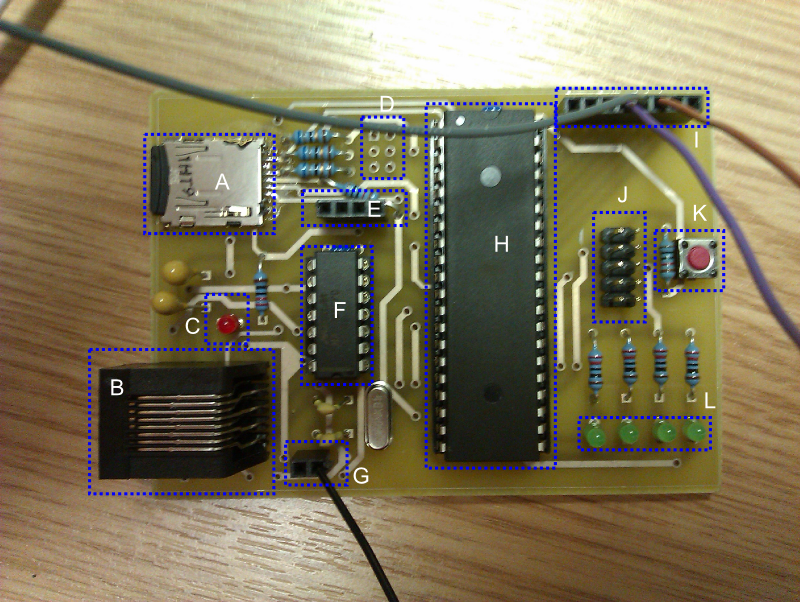
\includegraphics[width=1.00\textwidth]{figures/PayloadImplementation.png}
        \captionof{figure}{Image of the final payload, under test, before lacquer is applied. R11 can be seen between the Camera header and a via near the SD card Vcc.}. 
        \label{fig:PayloadImplementation}
\end{figure}

In figure \ref{fig:PayloadImplementation}, the letters refer to the following 
features of the payload module:

\begin{itemize}
\item \textbf{A:} microSD Card slot
\item \textbf{B:} RJ45 socket, more popularly known as an ethernet socket. 
(Actually implements the RS485 protocol)
\item \textbf{C:} Power LED. Shows whether 3V3 from the ethernet socket is connected.
\item \textbf{D:} ISP programming header socket. As seen, this is not 
soldered on, as we have been using the JTAG header for testing, but will be soldered 
before delivery to the customer.
\item \textbf{E:} Camera header. The camera can be connected to our PCB 
simply by attaching the hook-up wire in the correct order. (L-R: 3V3, GND, 
Camera TX, Camera RX)
\item \textbf{F:} MAX489 (RS485 Transceiver) \footnote{\url{http://uk.farnell.com/9725148}}. 
Cheaper version of the MAX3070 used in the sample peripheral.
\item \textbf{G:} Power header. L: 3V3, R: GND.
\item \textbf{H:} ATmega644P \cite{atmega644p}
\item \textbf{I:} ATmega644P Port A expansion header. (In the image, this is 
being used as a connection to an Arduino Uno so that we may view the debug 
information)
\item \textbf{J:} JTAG programming header
\item \textbf{K:} Reset button
\item \textbf{L:} Debug LEDs
\end{itemize}


%% ----------------------------------------------------------------
\chapter{Implementation - Ground Station}
%% ----------------------------------------------------------------

\label{chap:implementation_ground_station }

The user can only see the image viewer program.
In order to make the development faster, the console application has been use to test port send/receive information and convert the image data.
The programmer make use of both data stream port and the console port in order to send command and receive JPEG photo from the UAV.

\section{The development process} 
Because GUI include many functions on the application and also it links to TCP/IP ports, the GUI part consider as a very big program. 
Therefore, in order to complete the GUI step by step, it needs a plan for the development.
The connection to datastream can be done by using a console application describe in section\ref{sec:testing_connection_send_to_stream}.
If the connection is correct the appliction can listen to the data stream port as in section\ref{sec:testing_receive_stream}.
These console application will be combined to a bigger and more complete program in later section.

\flushleft
\begin{enumerate}


\item	The most important process of GUI development is to understand what does the customer wants. 

\item	The hardware and software specification have to be determined.
 
\item	Make a GUI design decision

\item Develop a smaller program in order to make the testing easy and less time consuming. 

\item	Learn the .NET class that can support the connection to TCP/IP, and communication between host and device

\item	Use GUI to link to the customer’s software to access the software

\item	Distribute the GUI
\end{enumerate}

\section{Use Case Diagram}
The use case diagram show what functionality the user can use in the program.
It has to include all the specification that the customer want for a complete system.
Figure~\ref{GUI_useCase} shows a possible user action on the program which the user can save, open and delete any jpeg image from the computer. 
The user has an option to connect to the UAV in case of the UAV is not connected properly.
He can command the image viewer program to send an image to the software, and it will display the image onto the picture box.
\begin{figure}[H]
\begin{center}
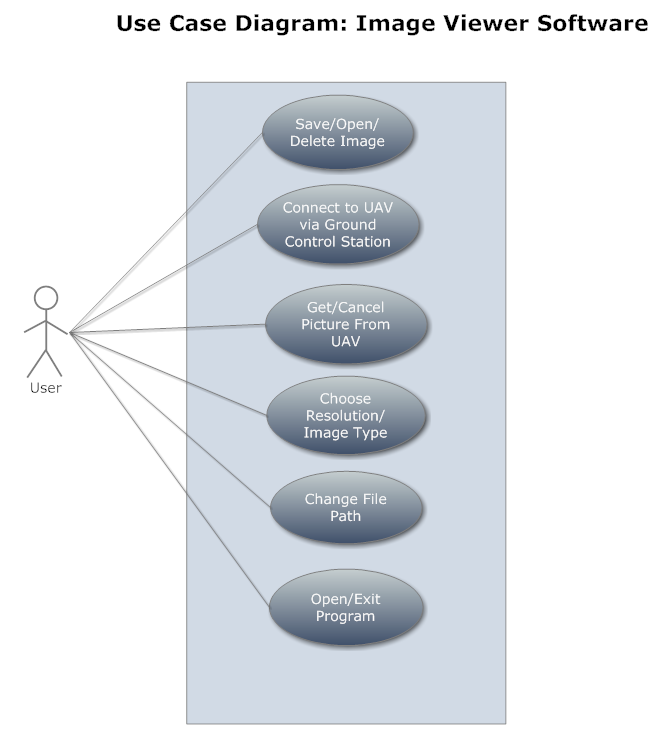
\includegraphics[scale=0.6]{figures/userCase.png} 
\end{center}
\caption{Use case diagram of the GUI\label{GUI_useCase}}
\end{figure}

This initial user diagram has changed because some of the action implement in the background. For example, connect to the UAV function, the user might be confused and click on this button every time the program is open. So the better way to implement this is to make the program connect to the UAV automatically when the program starts running. 
Another changes is the type of image implemented is JPEG only because the raw image will be too big so we decide not to implement it.
Therefore, the Milestone\ref{sec:ms_pl_img_gs_cam_colour_type} will not be implemented.
Figure\ref{GUI_finalUseCase} shows an agreed use case diagram. 

\begin{figure}[!hbtp]
\begin{center}
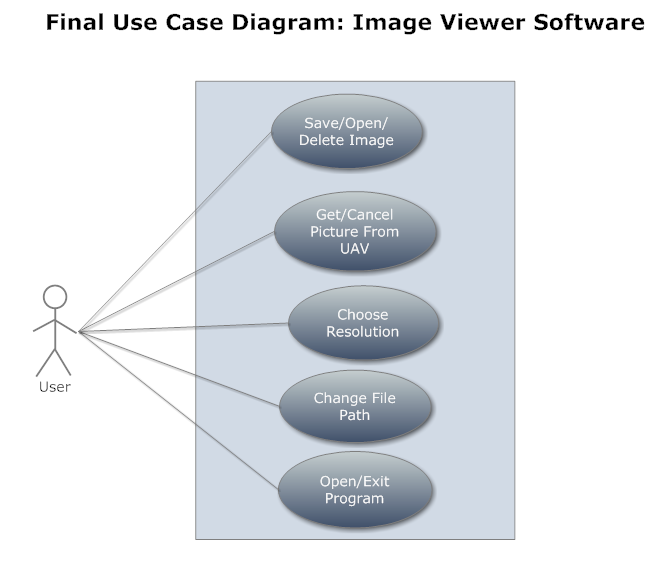
\includegraphics[scale=0.7]{figures/FinaluserCase.png} 
\end{center}
\caption{Final use case diagram of the GUI\label{GUI_finalUseCase}}
\end{figure}



\section{The Design}

The user for our application is assumed to have a limited programming experience, so the program will be implemented so it is simple understand. Figure~\ref{ini_GUI} show the first brainstorm view of the GUI. 
During the downloading process, the application should keep running so the cancel button can be used. 
Gallery button will link to another page which will be the collection of images taken. 
Left and right button can navigate the picture box to view an earlier picture or later picture. 
Cancel button cancel the receiving image, therefore the corrupted picture will not be downloaded. 
The user mode of the application can access only the main feature such as take picture, change directory, and cancel download picture.  
It allows the user to choose the resolution and picture type (RAW or JPEG) to transmitted from the UAV to the ground station. But the user doesn't have access to changing the command, changing the receiving data, and any interaction with the UAV because of safety and avoid of any errors. 
\begin{figure}[H]
\begin{center}
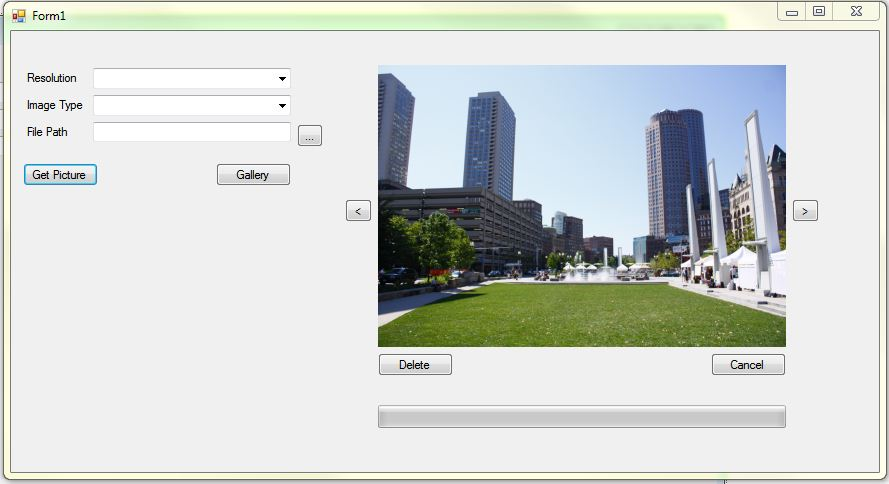
\includegraphics[width=1.0\textwidth]{figures/initialGUI.png} 
\end{center}
\caption{The initial design of GUI\label{ini_GUI}}
\end{figure}
The GUI has been planned to have functions such as auto triggering, image type, resolution type, file path chosen, progress bar, help button, stop and delete. Figure \ref{finalGUI} is the screen shot of the final GUI.

\begin{figure}[H]
\begin{center}
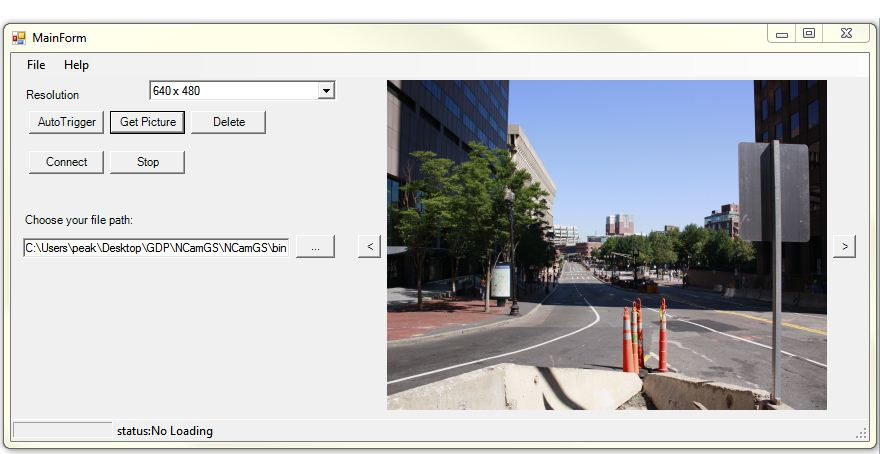
\includegraphics[width=1.0\textwidth]{figures/finalGUI.png} 
\end{center}
\caption{final GUI\label{finalGUI}}
\end{figure}

\section{Class Diagram}
\subsection*{The Initial Class Diagram}
Figure~\ref{ini_Class} shows initial classes and methods of the image viewer program.
The \texttt{JPEGFileReader} Class has functions for decoding/encoding the JPEG file.
There will be decoding/encoding algorithm because the image will take long time to download to the ground station. 
\begin{center}
\begin{figure}[!hbtp]
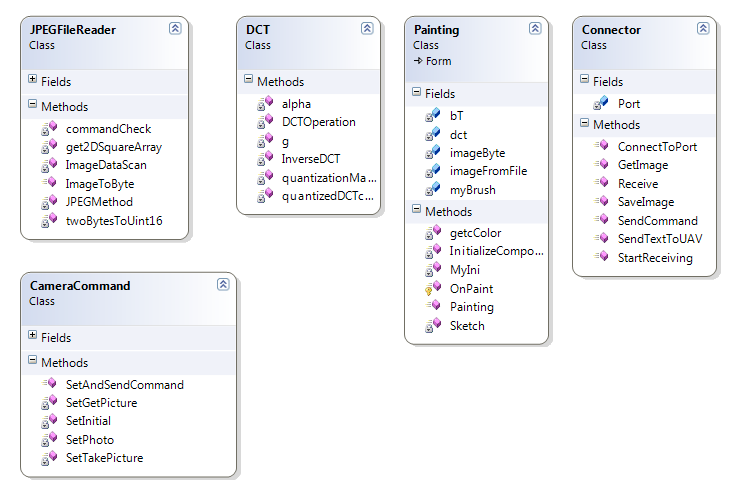
\includegraphics[width=150mm,height=100mm]{figures/initialClassDiagram.png} 
\caption{The initial design of GUI classes\label{ini_Class}}
\end{figure}
\end{center}
\texttt{DCT} class has many math operation and equation which have to be implemented on the image viewer program. 
This complicated function should implement in the ground station because if the picture is encoded in the compressed way, the ground station must be able to extract it. 
In the end, we have to determine whether it is faster to display image normally, or to do encoding/decoding JPEG file. 

The \texttt{Painting} class is supported by the \texttt{DCT} class. The intention of this class is to display an encoded image point by point on the \texttt{pictureBox}.
By this method, the \texttt{pictureBox} can display an image from the first pixel transmitted.

The \texttt{CameraCommand} class design for send the data from the ground station to the camera. The idea is that make the camera sync with the payload by using the ground station command. \texttt{SetAndSendCommand()} use for set the byte command and then send it to the payload via the Console port. \texttt{SetGetPicture(),SetInitial(), SetPhoto(), and SetTakePicture()} methods use for setting the correct byte in order to send the byte by using \texttt{SetAndSendCommand} class.

\subsection*{The Class Diagram}
The class diagram has been implemented very differently from the planned one.
This is because the new plan is to decode the image on board and then transmitted to the ground station in JPEG further compressed file. 
Therefore, the class \texttt{JpegFileReader} has changed to C code and to be implemented on board. 
The \texttt{DCT} class is not needed anymore because all the calculation will be on board. 
The \texttt{CameraCommand} has taken away because the payload will receive an image viewer command to the payload and then the payload will send another different signal to the camera.
Therefore, the command send to the camera from the payload does not have to be the same as the command sent from ground station to the payload. 
The \texttt{Painting} class use to draw each pixel onto the \texttt{pictureBox}, but it has not been implemented in the final program because of the stated reason.
Therefore, the milestone\ref{sec:ms_pl_img_gs_progressive_dl} will not be implemented.
This is also because of the time limitation.
More detail about the progressive image is in the section\ref{sec:implementation_progressive_jpeg}.
 
\begin{figure}[!hbtp]
\begin{center}
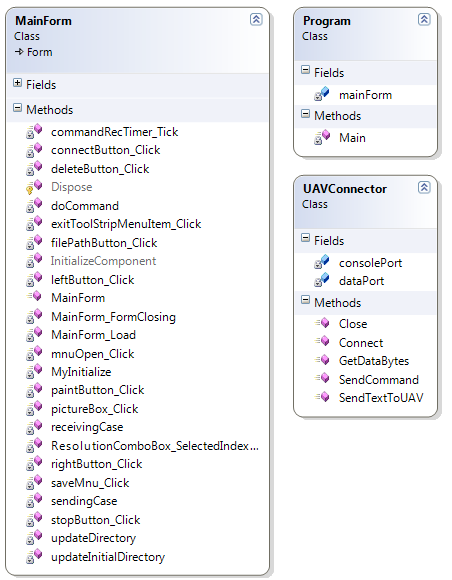
\includegraphics[scale=0.7]{figures/finalClassDiagram.png} 
\end{center}
\caption{Final class diagram of the GUI\label{GUI_finalClassDiagram}}
\end{figure}

\section{Before Connect to the Image Viewer Program}
Figure \ref{schemetic_clipA} shows a diagram of how the connection of the hardware should be. 
The UAV ground receiver is a USB-compatible device which uses Zigbee to communicate. 
USB device driver has been developed by the customer’s so the hardware can be accessed by ground station software, and other applications. 
USB is active when the host ask for a data. 
A host is the computer network which the UAV connect to. 
The data in its queue until the host asks for the data. 
\begin{figure}[!hbtp]
\begin{center}
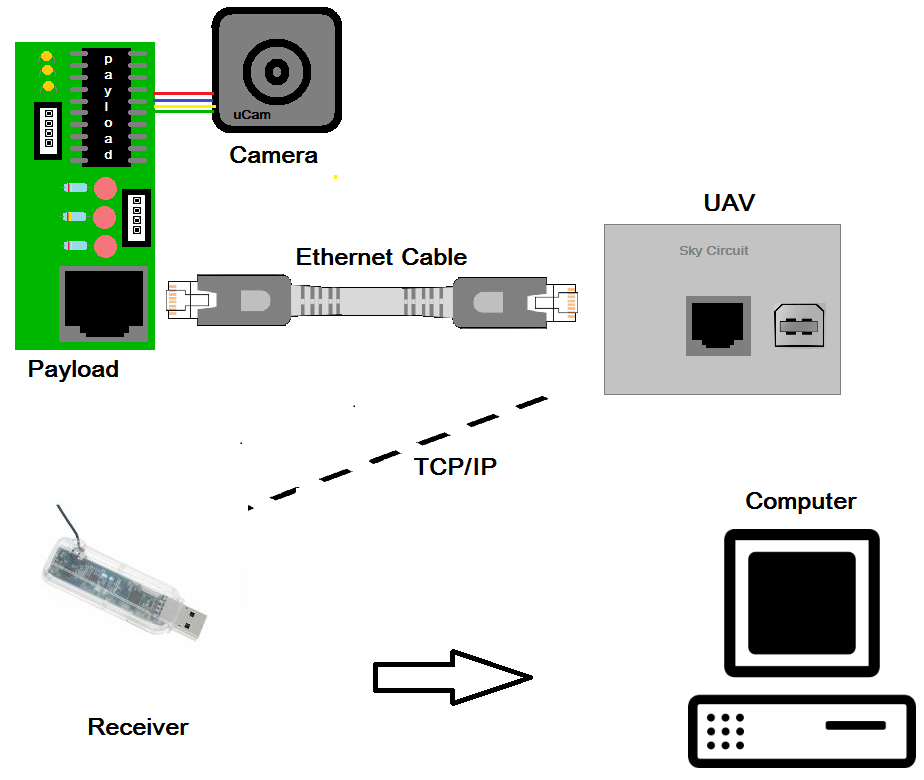
\includegraphics[scale=0.4]{figures/clipArt.png} 
\end{center}
\caption{The connection of the hardware\label{schemetic_clipA}}
\end{figure}


\section{GUI data flow diagram}

Table~\ref{command_table} shows how the command send and receive to/from ground station.  Figure~\ref{GCS_Payload_comm} give a brief detail of how the data communicate between the payload and the image viewer program. 
A more detailed diagram on the data communication is in figure \ref{sequence diagram}.
This has been tested in section\ref{sec:send_console}.

\begin{figure}[H]
\begin{center}
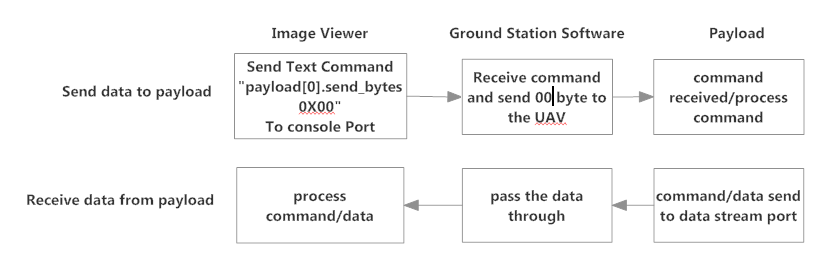
\includegraphics[scale=0.6]{figures/GCS_Payload_communication.png} 
\caption{The connection of data stream port\label{GCS_Payload_comm}}
\end{center}
\end{figure}

\begin{table}[H]

\begin{center}
\begin{tabular}{l l @{.} l}
 Command&
\multicolumn{2}{l}{Address Byte } \\

\hline
\underline{Command from Ground} & \\
SEND\_ZERO\_TOKEN & 0 \\
TAKE\_PICTURE & 0 \\
SEND\_DOWNLOAD\_REQUEST & 2 [MSB] [LSB]  \\
\\
\underline{Command received at Ground}\\
PICTURE\_TAKEN & 1 [MSB] [LSB]\\
DOWNLOAD\_INFO & 3 [MSB] [LSB]\\
IMAGE\_DATA & 4 $\overbrace{ [packet number]}^{2bytes} \overbrace{[image data]}^{data length}$ \\
\end{tabular}
\caption{Command table\label{command_table}}
\end{center}
\end{table}

\section{Get Image Algorithm}
\label{get image algorithm}
In order to take the picture and send it back to the ground station is very important and it has a complex signal algorithm to do.
The plan is when the user click on the Get Picture button, the program sends a \textbf{string command} to the ground station software.
Then the ground station software generates a \textbf{byte command} to transmitted by TCP to the payload. 
Then the payload sends a ''Picture Taken'' command back through the data stream port to the Image Viewer Program. 
Picture taken button has been tested in section\ref{sec:test_get_image_button}
The Image Viewer Program will then automatically send a download request command to the payload. 
The payload will then send image data back to the data stream port. 

When the program start running, the program initialized the port and commands the customer’s application to tell the UAV to stream data to the data stream port. Figure~\ref{GCS_connect_command} shows the connection between the UAV data stream port and the ground station. The UAV has two ports, console port, and data stream port and it can send and receive any length of data. There are some global initializations that the software needs to perform only once when it is loaded for the first time. Note that the console port is manually connected by the ground control station software. The image viewer will give a warning in message box when there is no connection.

\begin{figure}[!hbtp]
\begin{center}
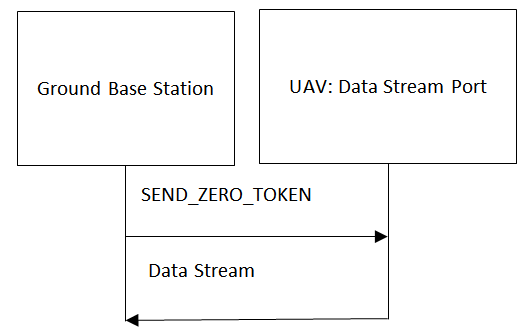
\includegraphics[scale=0.5]{figures/connect_command.png} 
\end{center}
\caption{The connection of data stream port\label{GCS_connect_command}}
\end{figure}


 
\section{Code Highlight}

This section describes the code that is important for the program. The entire code will not be described but it will be in the appendices. It needs a class that can do these to port: connect, receive and send. \texttt{FileStream} class is a class in the .NET C\# which can create a file. \texttt{BinaryWriter} class is use for writing the byte data into a specific file made by the \texttt{FileStream} class. The file directory will introduce a thread. While the open or save a file, the main application must be running, so the application needs to deal with multi threads at the same time. Also when the get picture button got clicked, the main application is frozen because of the thread time organize do one thing at a time. 

\subsubsection*{Connect to UAV:Appendix \ref{appen:UAVConnector} line 18-38.}
The \texttt{Socket} class has functions to send and receive byte and strings data. The handshaking protocol is using \texttt{PortConnect()} method.  
        
The design of the .NET \texttt{Socket} class simply connects to a Port by a single command without any hesitation of changing the baud rate, stop bits, and parity bits. 
This advantage makes the \texttt{Socket} class a more useful class then the \texttt{SerialPort} Class to work with the Port with existing and static set up. 
This class has been tested using a console application before implementing it in a final GUI. 
This will complete milestone\ref{sec:ms_pl_tx_token_resp}.

\subsection{Start of the program: Appendix \ref{appen:main_form} line 78-87}%
In order to make the file name different and meaningful, the name of the picture will be the time and date of the time taken the picture. The code \texttt{DateTime.Now} generate a string of date and time of the current time. This has been done using the date and time class. \texttt{FileStream} was initialize to be in \texttt{FileMode.Create()}, so it can create file. The BinaryWriter write the binary byte into a file in the directory of the fileStream. \texttt{string fileName = string.Format("uavPictureAt{ 0 : yyyy-MM-dd\_ hh-mm-ss-tt}
 .jpg", DateTime.Now);   }  
This code time setting is valid for a file name because it is not using any symbol that will make the program confuse with a code. 
It will display year, month, date, and time in this order. 
The \texttt{BinaryWriter} class can create a binary file using specific data layout for its bytes. 


\subsection{Text Command:Appendix\ref{appen:UAVConnector} line 68-85}
TCP/IP protocols transfer data without modifying them. This allow the application to freely encode the data.\cite{davidB}.The Ground station software allow the program to send a stream of string in bytes and it will read the command bytes and send it to the payload on the UAV. The code has shown the way to implement the string and send a byte array to the payload.

To send text, the string of characters is translated into an array of bytes. American Standard Code for Information Interchange(ASCII) is use for translating English into a binary code. In the \texttt{System.Text} classes provide converting mechanism between each character sets. The \texttt{ASCIIEncoding.GetBytes()} is used for convert character array into a byte array.  
\texttt{The Socket.Send()} method allows the user to send byte stream to the port connected. The customer's program will read from the port and display it onto the command line. The ''@ '' sign indicate that the command correctly sent from the application to the ground station software. The advantage of linking to the ground station software is that our customers can understand what is going on in the console line. For example:uavConn.SendTextToUAV(''da 20 payload[0].mem\_ bytes[0]'');
\ref{sec:ms_pl_shared_mem_set}

The text \texttt{''da 20 payload[0].mem\_ bytes[0]''} will be converted to char array and then to byte array. The byte array will then send the command to the console port to the payload by \texttt{consolePort.Send(toUAVByte, toUAVChar.Length)}. The customer is familiar with the ground station software program, so he can understand the background of the transmission as well. This will complete Milestone\ref{sec:ms_pl_rx_msg_gs}.

In order to test that the payload receives the same data, we use the oscilloscope to see the signal. The byte display on the payload is the same as the byte data send from the ground station. Therefore, the Milesone\ref{sec:ms_pl_img_gs_trigger} is completed. The different resolutions send different byte command to the payload. The byte command changes if the comboBox options change. Therefore, we can say that Milestone\ref{sec:ms_pl_img_gs_cam_res} has completed.


\begin{lstlisting}[caption={writing binary file},label=lst:writingb]          
	for (int i = 3; i < packetSize; i++)
	{
          opFile.Write(packet[i]);
          numBytes++;
    	}
\end{lstlisting}         

At every cycle of the data being received, \texttt{opFile.Write()} method will write the packet data into the file in the directory. After the cycle finished, the file will be saved and the image will be displayed in the picture box. 

\subsection{Get Picture Button}
This get picture button will use both send and receive function of the program. 
The work flow of the get picture signal show in figure \ref{GUI_finalWorkFlow}.
If the sequence of signal send/receive correctly, the photo that receive from the sky will be display on the photo box in the program.
This will complete Milestone\ref{sec:ms_pl_img_sending_gs}.

\begin{figure}[H]
\begin{center}
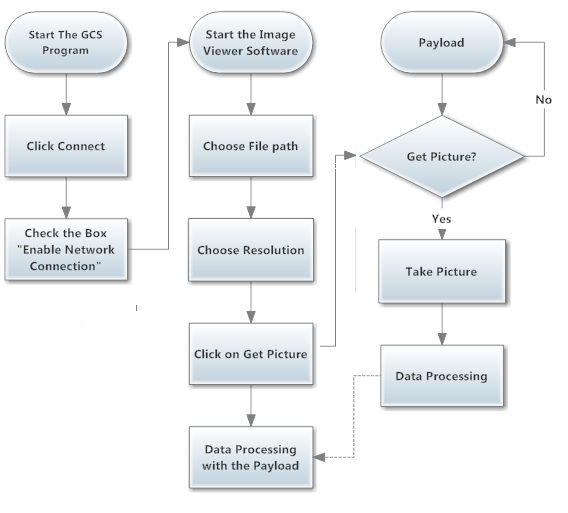
\includegraphics[scale=1]{figures/finalWorkFlow.png} 
\end{center}
\caption{Final work flow diagram of the GUI\label{GUI_finalWorkFlow}}
\end{figure}

\subsection{Implementation - Way-point Triggering (ms)}
\label{sec:waypoint_triggering}

\subsubsection{Description}

The ground station is capable of assigning way-points to
the payload which will allow the camera to take pictures 
at a given location.

This is achieved by sending a simple command script from
the ground station to be uploaded by the payload 
controller. The way-point is designated by the user
through the ground station software. The script 
tells the UAV controller to continuously check the
distance separating itself from the way-point.
When the UAV reaches is within 200 metres of the
way-point, a 0 byte is sent to the camera to prompt
the camera to take a picture.

After taking a picture at the way-point, the camera
is delayed for 10 seconds to avoid taking another picture
at the same way-point. When the 10 second delay is over,
the camera repeats the operation and continuously checks
its distance from the next waypoint.

\subsubsection{Pseudo-code description}

Below is a brief pseudo-code description of the script
sent by the ground station to the payload to take an
image at designated way-points:

\begin{itemize}
	\item while !(UAV distance from next way-point $le$ 200 metres)
		\begin{itemize}
			\item Do nothing.
		\end{itemize}
	\item end while
	\item Prompt camera to take an image.
	\item wait 10 seconds
	\item Re-enter while loop
\end{itemize}

\subsection{Other functions}
The user might want to delete some unwanted photo, so the delete button have been implemented. The delete button work like a normal file deleting button. But it has been complicated because the photo to delete must be the photo on the pictureBox. There is an error because the photo is using by the pictureBox. To fix this problem, the picture have to shifted left or right first and then delete the photo. But where there is only one picture in the file, the program is not allow to delete because even the pictureBox is set to null, its last memory is still point at the deleting file. However, the disadvantage of the delete button is that if the wanted photo got deleted accidentally, it might take a long time to launch the UAV again and take the same photo. The program can also detect the corrupted image and ask the user to delete it.

\begin{figure}[H]
\begin{center}
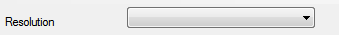
\includegraphics[scale=0.5]{figures/resolutionOption.png} 
\end{center}
\caption{The resolution in combo box\label{resolutionOption}}
\end{figure}
The camera has options of resolution as shown in Figure\ref{resolutionOption}. This can be useful when the speed is important. The lower the resolution, the faster the data transmitted to the ground. GUI has the combo box for the user to choose any wanted resolution in the options. The resolution allow user to have more accessible to the camera. However, this mean there is more on the programmer side to program the application.


It takes around 8 to 20 seconds to transmit an image of resolution 640x480. This progress bar tells the user how much percentage of data received. The progress bar update at each cycle of the data receives. The status text tells the user what signal have been sent or received. Figure\ref{progressBar} shows the status text ensures that the picture is downloading. However, these have to implement every cycle of the data collection and it might cause the cycle to run slower. The actual loop is much faster than the 38.4kbaud, therefore there is no problem implementing these in.
\begin{figure}[H]
\begin{center}
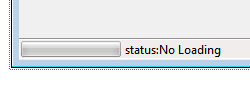
\includegraphics[width=0.3\textwidth]{figures/progressBar.png} 
\end{center}
\caption{The resolution in combo box\label{progressBar}}
\end{figure}

\section{Complete System}
After all the implementation has completed, all the function will be tested together. All the smaller program that we have implemented will be combined at this stage. The send and receiving will use to implement the communication between the payload and the Image Viewer Software. The display of image data will implement as a final display of the image.  Figure \ref{completeSystem} shows a final working GUI of our program. 
\begin{figure}[H]
\begin{center}
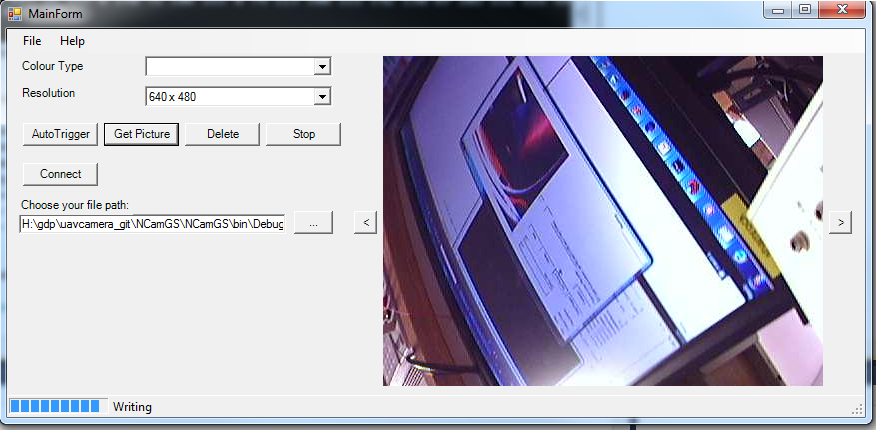
\includegraphics[width=1.0\textwidth]{testing_screenshots/ui.png} 
\end{center}
\caption{The complete system\label{completeSystem}}
\end{figure}




%% ----------------------------------------------------------------
\chapter{Implementation - Whole System}
%% ----------------------------------------------------------------

\section{System Integration}

